%------------------------------------------------------------
%
\documentclass[a4paper,12pt,reqno,oneside]{amsart}
%
%----------------------------------------------------------
% This is a sample document for the AMS LaTeX Article Class
% Class options
%        -- Point size:  8pt, 9pt, 10pt (default), 11pt, 12pt
%        -- Paper size:  letterpaper(default), a4paper
%        -- Orientation: portrait(default), landscape
%        -- Print size:  oneside, twoside(default)
%        -- Quality:     final(default), draft
%        -- Title page:  notitlepage, titlepage(default)
%        -- Start chapter on left:
%                        openright(default), openany
%        -- Columns:     onecolumn(default), twocolumn
%        -- Omit extra math features:
%                        nomath
%        -- AMSfonts:    noamsfonts
%        -- PSAMSFonts  (fewer AMSfonts sizes):
%                        psamsfonts
%        -- Equation numbering:
%                        leqno(default), reqno (equation numbers are on the right side)
%        -- Equation centering:
%                        centertags(default), tbtags
%        -- Displayed equations (centered is the default):
%                        fleqn (equations start at the same distance from the right side)
%        -- Electronic journal:
%                        e-only
%------------------------------------------------------------
% For instance the command
%          \documentclass[a4paper,12pt,reqno]{amsart}
% ensures that the paper size is a4, fonts are typeset at the size 12p
% and the equation numbers are on the right side
%
\usepackage{amsmath}%
\usepackage{amsfonts}%
\usepackage{amssymb}%
\usepackage{tikz}
\usetikzlibrary{calc,trees,positioning,arrows,fit,shapes,calc}
\usepackage{graphicx}
\usepackage{hyperref}
\usepackage{amssymb}
\usepackage{amsmath,amsthm}
%------------------------------------------------------------
% Theorem like environments
%
\newtheorem{theorem}{Theorem}
\theoremstyle{plain}
\newtheorem{acknowledgement}{Acknowledgement}
\newtheorem{algorithm}{Algorithm}
\newtheorem{axiom}{Axiom}
\newtheorem{case}{Case}
\newtheorem{claim}{Claim}
\newtheorem{conclusion}{Conclusion}
\newtheorem{condition}{Condition}
\newtheorem{conjecture}{Conjecture}
\newtheorem{corollary}{Corollary}
\newtheorem{criterion}{Criterion}
\newtheorem{definition}{Definition}
\newtheorem{example}{Example}
\newtheorem{exercise}{Exercise}
\newtheorem{lemma}{Lemma}
\newtheorem{notation}{Notation}
\newtheorem{problem}{Problem}
\newtheorem{proposition}{Proposition}
\newtheorem{remark}{Remark}
\newtheorem{solution}{Solution}
\newtheorem{summary}{Summary}
\numberwithin{equation}{section}

\hypersetup{pdftitle={MDS Scribing}}
%--------------------------------------------------------
\begin{document}
\title[Rank Nullity Theorem and Matrix Representation]{Lecture 5 and 6}

\author{Shubh Agarwal}
 \email[Shubh]{210020047@iitdh.ac.in}%
 \urladdr{https://shubhagarwal-dev.github.io/}

 \author{Saksham Chhimwal}
 \email[Saksham]{210010046@iitdh.ac.in}%
% %\urladdr{http://www.authortwo.uni-atwo.hu}

 \author{Abhiram K}
 \email[Abhiram]{210150001@iitdh.ac.in}%

\author{Rishabh Sharad}
\email[Rishabh]{210020036@iitdh.ac.in}%

%\thanks{Thanks for Author One.}
%\thanks{Thanks for Author Two.}
\thanks{This paper is in final form}
\date{\today}
\subjclass{2023 Mathematics for Data Science, CS-427} %
%\keywords{Keyword one, keyword two etc.}%
%\begin{abstract}
%This is a sample document which shows the most important features of the AMS Journal
%Article class.
%\end{abstract}
\maketitle

\section{Rank Nullity Theorem}
It is also called then fundamental theorem of Linear Maps because of its importance
in linear transformation.

\subsection{Statement and Proof}

\begin{theorem}
	\textbf{Rank-Nullity Theorem:}
	Suppose V is finite-dimensional and $T\in\mathcal{L}:(V, W).$ Then range T is 
	finite-dimensional and 
	\begin{center}
		$Rank(T)$ + $Nullity(T)$ = $\dim(V)$, or
	\end{center}
	\begin{center}
		$\dim(Range(T))$ + $\dim(Ker(T))$ = $\dim(V)$
	\end{center}
\end{theorem}

\begin{proof}[Proof]
	
	Let $\phi_1,\phi_2,\ldots,\phi_l$ be the minimum vectors will that span $Ker(T)$, where l is the \dim(Ker(T)).\\
	And $v_1, v_2, \ldots, v_{n-l}$ be the vectors that will span the remaining vector space $V$ where, $n$ is the \dim(V).$
	Their linear transformation \\($w_1, w_2, \ldots, w_{n-l} $) must be independent and should span the entire range of
	$T$ in $W$, let $\dim(Range(T))$ be $k$.
	
	\emph{We will prove this claim later}.\\
	Then it becomes quite easy to see why the rank nullity theorem holds.\\
	Because,
	$$
		n-l=k \,\,\,or\,\,\, n=l+k
	$$
	Hence, Proved.
\end{proof}

	\begin{claim}
		$w_1, w_2, \ldots, w_{n-l}$ are linearly independent and span the entire $Range(T)$.
	\end{claim}
	\begin{proof}[Proving Claim]
	$w_1, w_2, \ldots, w_{n-l}$ are linear transformation of basis \\ $v_1, v_2, \ldots, v_{n-l}$.
	So,
	\begin{eqnarray*}
		\alpha_1  w_1 + \alpha_2 w_2 + \ldots + \alpha_{n-l} w_{n-l} & = & 0 & \\
		or, \sum_{i=1}^{n-l}{\alpha_i w_i} & = & 0 &\\
		or, \sum_{i=1}^{n-l}{\alpha_i Tv_i} & = & 0 &\\
		or, T(\sum_{i=1}^{n-l}{\alpha_i v_i}) & = & 0 &\\
	\end{eqnarray*} 
	So $ \alpha_1  v_1 + \alpha_2 v_2 + \ldots + \alpha_{n-l} v_{n-l} $ \in \dim(null T).\\
	Since, $\phi_1,\phi_2,\ldots,\phi_l$ spans \emph{null T}, we can write:
	$$
		\alpha_1  v_1 + \alpha_2 v_2 + \ldots + \alpha_{n-l} v_{n-l} = \beta_1 \phi_1 + \beta_2 \phi2 + \ldots + \beta_l \phi_l
	$$
	But we also know that $\phi_1 \, to \, \phi_l$ and $v_1 \, to \, v_{n-l}$ are linearly independent, which means the onlu way to satisfy above
	equation is to have \alpha_1=\alpha_2= \ldots=\alpha_{n-1}=\beta_1=\ldots=\beta_l = 0.\\
	Thus $Tv_1, Tv_2,\ldots, Tv_{n-l}$ are linearly independent and span the entire $Range(T)$.
	Hence $w_1, w_2, \ldots, w_{n-l}$ will span the entire $Range(T)$.
  \end{proof}

\subsection{Applications}

We can now prove that some of the mapping can not be surjective or injective.
\begin{theorem}[A map to a smaller dimensional space is not injective]
	Suppose $V$ and $W$ are finite-dimensional vector spaces such that $\dim(V)$ and
	\gtr $\dim(W)$, then there is no injective linear mapping from $V$ to $W$.
\end{theorem}

\begin{proof}[Proof]
	Let $T\in\mathcal{L}$:($V$, $W$). Then
	%\begin{center}
	%$\dim(null$ $T$) = $\dim(V)$ - $\dim(Range (T))$ \newline
	%$\dim(null$ $T$) > $\dim(V)$ - $\dim(W)$ \newline
	%$\dim(null$ $T$) \geq $0$
	%\end{center}
	\begin{eqnarray*}
	\dim(null\,T)&=&\dim(V) - \dim(Range (T)) \\
	& \geq & \dim(V) - \dim(W) \\
	& > & 0
	\end{eqnarray*}
	
	The equality above comes from the fundamental theorem of Linear Maps and the strict inequality at the end shows the dimension of T is greater than 0, means vector other than 0 are present in T. Hence the mapping is not injective.
\end{proof}

\begin{theorem}[A map to a larger dimensional space is not surjective]
Suppose $V$ and $W$ are finite-dimensional vector spaces such that \dim(V) and
	\ltr $\dim(W)$, then there is no surjective linear mapping from $V$ to $W$.
\end{theorem}
\begin{proof}[Proof]
	Let $T\in\mathcal{L}$:($V$, $W$). Then
	\begin{eqnarray*}
	\dim(range\,T)&=&\dim(V) - \dim(null\,T) \\
	& \leq & \dim(V) \\
	& < & \dim(W)
	\end{eqnarray*}
	Here again the equality comes from the Rank-Nullity Theorem, and the rest is just normal inference.\\
	At the end we have range of T < the dimension of W. Hence the mapping is not surjective.
\end{proof}
\section{Matrix Representation of Linear Transformation}
A vector is represented in different ways on the coordinate system depending on what its basis is. Suppose the vector (2,1) in $R^2$ is represented with basis as 
$\begin{pmatrix}
    1 & 0\\
    0 & 1
\end{pmatrix}$


 \begin{center}
     \includegraphics{"figure1.jpg"}
 \end{center}
 
 But when the basis is changed the vector is represented differently and on a different basis.
 \newline
 The vector $V$ can be represented as $a_{1} b_{1} + a_{2} b_{2}$ and in matrix form can be represented as $V \begin{pmatrix}
     a_{1}\\
     a_{2}
 \end{pmatrix}$.
 \newline
 Suppose there are is a linear transformation $T$ that maps a vector $V$ from $R^{n}$ to $W$ in $R^{m}$.
 Let the basis be $B= \{e_{1},\dots ,e_{n}\}$ and $B^\prime = \{e_{1}^\prime , \dots ,e_{m}^\prime \}$
 The map can be represented as 
 \begin{center}
 \centering
 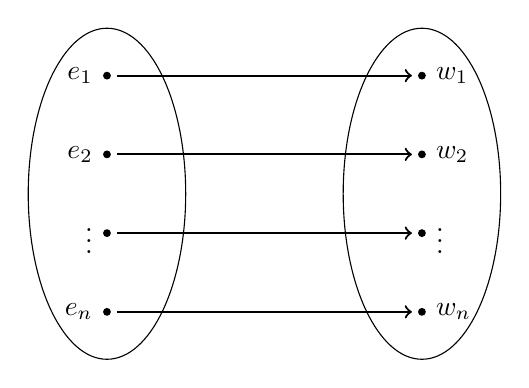
\begin{tikzpicture}[ele/.style={fill=black,circle,minimum width=.8pt,inner sep=1pt},every fit/.style={ellipse,draw,inner sep=-2pt}]
  \node[ele,label=left:$e_{1}$] (a1) at (0,4) {};    
  \node[ele,label=left:$e_{2}$] (a2) at (0,3) {};    
  \node[ele,label=left:$ \vdots $] (a3) at (0,2) {};
  \node[ele,label=left:$e_{n}$] (a4) at (0,1) {};

  \node[ele,,label=right:$w_{1}$] (b1) at (4,4) {};
  \node[ele,,label=right:$w_{2}$] (b2) at (4,3) {};
  \node[ele,,label=right:$ \vdots $] (b3) at (4,2) {};
  \node[ele,,label=right:$w_{n}$] (b4) at (4,1) {};

  \node[draw,fit= (a1) (a2) (a3) (a4),minimum width=2cm] {} ;
  \node[draw,fit= (b1) (b2) (b3) (b4),minimum width=2cm] {} ;  
  \draw[->,thick,shorten <=2pt,shorten >=2pt] (a1) -- (b1);
  \draw[->,thick,shorten <=2pt,shorten >=2] (a2) -- (b2);
  \draw[->,thick,shorten <=2pt,shorten >=2] (a3) -- (b3);
  \draw[->,thick,shorten <=2pt,shorten >=2] (a4) -- (b4);
 \end{tikzpicture}
 \end{center}
Suppose the basis for $B$ is $\begin{pmatrix}
    \alpha_{1}\\
    \vdots \\
    \alpha_{n}
\end{pmatrix}$ and the upon applying the transformation the basis for $B^\prime$ is $\begin{pmatrix}
    \beta_{1} \\
    \vdots \\
    \beta_{m}
\end{pmatrix}$
\newline
Now the question is how should we connect $\alpha_{i}$ to the $\beta_{j}$ such that we reach to our answer.
$$
\begin{array}
\\
    & \text{ We know that } Tv = w 
    & v = \sum_{i=1}^{n}\alpha_{i}e_{i} 
    & \text{Applying linear transformation T on both sides we get} 
    & Tv = \sum_{i=1}^{n}\alpha_{i}T \left( e_{i} \right) 
    \\
    & \text{Now what is $Te_{i}$ ?}
    &\text{In this case $e_{i} \rightarrow{} w_{i}$} 
    \\
    & \therefore Tv = \sum_{i=1}^{n}\alpha_{i}w_{i}
\end{array}
$$
But we want $w_{i}$ to be represented in terms of Standard Basis. \newline
$$
\begin{array}{cc}
    w_{i} = \begin{pmatrix}
        w_{1i}\\
        w_{2i}\\
        \vdots \\
        w_{mi}
    \end{pmatrix}
    \left( \text{This is the representation of $w_{i}$ in standard basis} \right) \\
    \therefore w_{i} = \sum_{i=1}^{m} w_{ij} e^\prime_{j}
    \end{array}
$$
Hence now the $Tv$ can be transformed as follows 
$$
\begin{array}{cc}
     Tv  =&  \sum_{i=1}^{n} \sum_{j=1}^{m} w_{ij} e_{j} \\
     Tv  =& \sum_{j=1}^{m} \left( \sum_{i=1}^{n} w_{ij} \alpha_{i} \right) e^\prime_{j} \\
     & \text{ Call the quantity } \left( \sum_{i=1}^{n} w_{ij} \alpha_{i} \right) = \beta_{j} \\
     \therefore Tv =& \sum_{j=1}^{m}\beta_{j} e^{\prime}_{j}\\
\end{array}
$$
This can now be represented in the matrix form as follows
$$
Tv = 
\begin{pmatrix}
    w_{1,1} & w_{1,2} &\cdots & w_{1,n} \\
    \vdots & \vdots & \vdots & \vdots \\
    w_{m,1} & w_{m,2} &\cdots & w_{m,n} 
\end{pmatrix}
\begin{pmatrix}
    \alpha_{1} \\
    \vdots \\
    \alpha_{n}
\end{pmatrix}
$$
Here we can clearly see that $Te_{i} = \left(\begin{matrix}
        w_{1,i} \\
        \vdots \\
        w_{m,i}
    \end{matrix}
\right)
    \text{That is the $i^{\text{th}}$ column in the matrix.}
$
Hence to get the first column and eventually $Te_{1}$ we must place the $\begin{pmatrix}
    \alpha_{1} \\
    \vdots \\
    \alpha_{n}
\end{pmatrix}$ equal to $\begin{pmatrix}
    1 \\
    0 \\
    \vdots \\
    0
\end{pmatrix}$. Similarly to get the second column we must place the $\begin{pmatrix}
    \alpha_{1} \\
    \vdots \\
    \alpha_{n}
\end{pmatrix}$ equal to $\begin{pmatrix}
    0 \\
    1 \\
    \vdots \\
    0
\end{pmatrix}$ and so on.
\newpage
\textbf{Example 1:} $\mathbb{R}^{2} \xrightarrow{T} \mathbb{R}^{2}$. Given 
\\
\begin{center}
\begin{pmatrix}
    1 \\
    2
\end{pmatrix} $\xrightarrow{T}$ \begin{pmatrix}
    -3 \\
    1
\end{pmatrix}
\\
\begin{pmatrix}
    -3 \\
    1
\end{pmatrix} $\xrightarrow{T}$ \begin{pmatrix}
    1 \\
    2
\end{pmatrix}
\end{center}
Find the linear transformation $\begin{pmatrix}
    \alpha_{1} \\
    \alpha_{2}
\end{pmatrix} \xrightarrow{T} \begin{pmatrix}
    \beta_{1} \\
    \beta_{2}
\end{pmatrix}.$
\newline
\newline
\textbf{Solution: }
The first question that arises is where the standard basis goes. The vector on the LHS be in the standard basis $\left( 1,0 \right)$ and $\left( 0,1 \right)$.
$$
\begin{array}{cc}
     \begin{pmatrix}
         1 \\
         2
     \end{pmatrix}
     \xrightarrow{T}
     \begin{pmatrix}
         -3 \\
         1
     \end{pmatrix}
     \\
     -2 \cdot \left(
     \begin{pmatrix}
         -3 \\
         1
     \end{pmatrix}
     \xrightarrow{T}
     \begin{pmatrix}
         1 \\
         2
     \end{pmatrix}
     \right)
	 \\
     = \begin{pmatrix}
         7 \\
         0
     \end{pmatrix}
     \xrightarrow{T}
     \begin{pmatrix}
         -5 \\
         -3
     \end{pmatrix}
     \\
     \implies \begin{pmatrix}
         1 \\
         0
     \end{pmatrix}
     \xrightarrow{T}
     \frac{1}{7}
     \begin{pmatrix}
         -5 \\
         -3
     \end{pmatrix}
\end{array}
$$
Similarly we find for the vector $\begin{pmatrix}
    0 \\
    1
\end{pmatrix}$ and we get it to be $\begin{pmatrix}
    0 \\
    1
\end{pmatrix} \xrightarrow{T} \frac{1}{7}\begin{pmatrix}
    -8 \\
    5
\end{pmatrix}$.
\\
Now we know the linear transformation for both the standard basis vectors. Now we can push these values in the matrix and get the value for the corresponding $\beta$ depending on the value of $\alpha$.
$$
\begin{pmatrix}
    \beta_1 \\
    \beta_2
\end{pmatrix} = \begin{pmatrix}
    \frac{-5}{7} & \frac{-8}{7} \\
    \frac{-3}{7} & \frac{5}{7}
\end{pmatrix} \begin{pmatrix}
    \alpha_1 \\
    \alpha_2
\end{pmatrix}
$$

%This text is a sample for a short bibliography. You can cite a book by making use of
%the command \verb"\cite{KarelRektorys}": \cite{KarelRektorys}. Papers can be cited
%similarly: \cite{Bertoti97}. If you want multiple citations to appear in a single set
%of square brackets you must type all of the citation keys inside a single citation,
%separating each with a comma. Here is an example: \cite{Bertoti97, Szeidl2001,
%Carlson67}.

%\begin{thebibliography}{9%
%\bibitem {KarelRektorys}Rektorys, K., \textit{Variational methods in Mathematics,
%Science and Engineering}, D. Reidel Publishing Company,
%Dordrecht-Hollanf/Boston-U.S.A., 2th edition, 1975

%\bibitem {Bertoti97} \textsc{Bert\'{o}ti, E.}:\ \textit{On mixed variational formulation
%of linear elasticity using nonsymmetric stresses and displacements}, International
%Journal for Numerical Methods in Engineering., \textbf{42}, (1997), 561-578.

%\bibitem {Szeidl2001} \textsc{Szeidl, G.}:\ \textit{Boundary integral equations for
%plane problems in terms of stress functions of order one}, Journal of Computational and
%Applied Mechanics, \textbf{2}(2), (2001), 237-261.

%\bibitem {Carlson67}  \textsc{Carlson D. E.}:\ \textit{On G\"{u}nther's stress functions
%for couple stresses}, Quart. Appl. Math., \textbf{25}, (1967), 139-146.
%\end{thebibliography}
\end{document}